\begin{answer}
\begin{figure}[H]
	\centering
	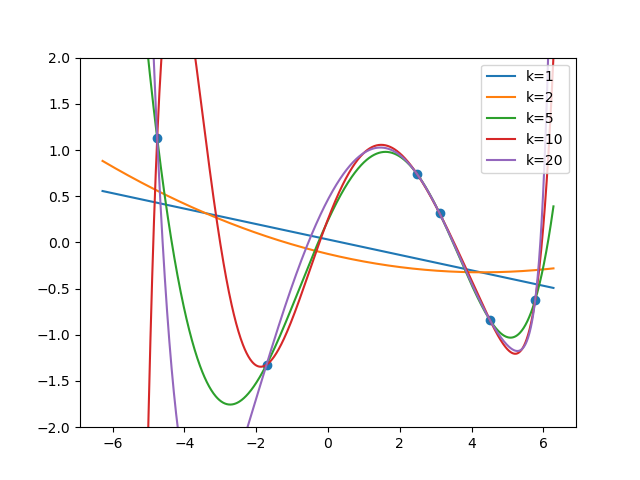
\includegraphics[height=0.25\textheight]{overfit}
	\caption{Small dataset.}
\end{figure}
There are only 6 examples on this dataset. The model perfectly explains these examples when $k \ge 5$. But the pattern becomes "unnatural" and doesn't look like of a sine function when $k = 20$. That's indication of overfitting.\\
\end{answer}
